\section{Confronto tra veicolo Ego in condizioni di Good e Bad Weather}
Per valutare l'impatto delle condizioni meteorologiche sul comportamento del sistema ACC, 
è stata condotta un'ulteriore simulazione mantenendo gli stessi parametri dei test precedenti, 
ma impostando la variabile \texttt{bad\_weather} a zero (condizioni meteorologiche pessime).
\\\\
\noindent In Figura \ref{fig:ego_acceleration_bw} è riportato il confronto tra l'\texttt{ego\_acceleration} 
nei due scenari (linea blu per \texttt{good\_weather} e linea gialla per \texttt{bad\_weather}).
\begin{figure}[H]
    \centering
    \adjustbox{center}{
        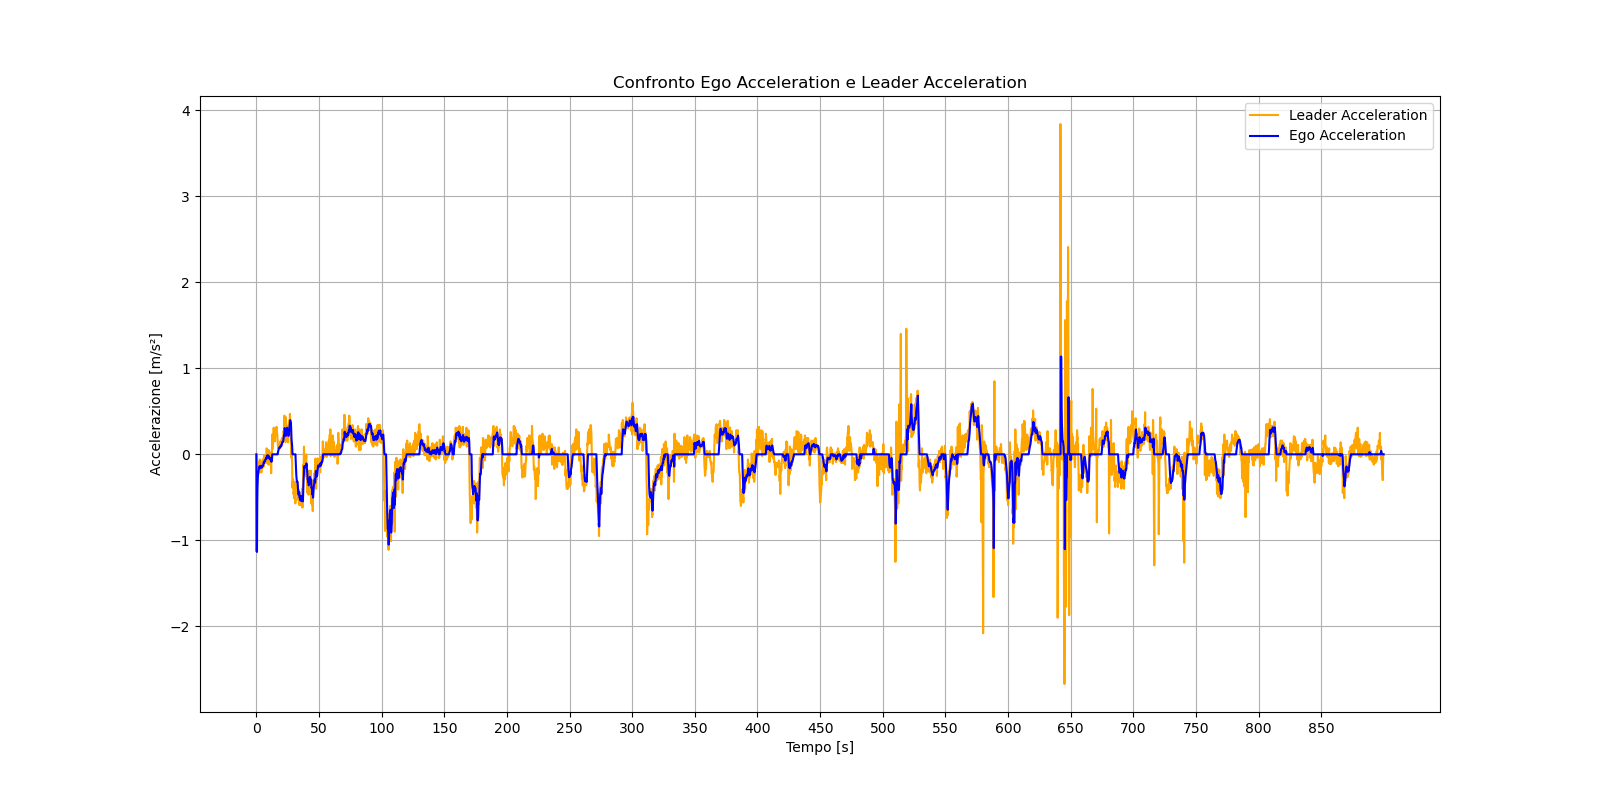
\includegraphics[width=1.25\linewidth]{simulation/bad_weather_ego_comparison/acceleration.png}
    }
    \caption{Confronto Ego Acceleration Simulata}
    \label{fig:ego_acceleration_bw}
\end{figure}
\noindent Le curve risultano quasi perfettamente sovrapposte, con una correlazione di Pearson pari a \textbf{0.922}. 
Le principali differenze si osservano nei picchi di decelerazione, più accentuati in condizioni di maltempo: 
in tali situazioni il sistema ACC tende infatti a incrementare lo \texttt{space\_gap}, generando frenate più marcate. 
Inoltre, all'inizio della simulazione, il veicolo in condizioni di \texttt{bad\_weather} mostra una
decelerazione significativamente maggiore, adottando una strategia di maggiore prudenza.
\\\\
\noindent Analogamente, la Figura \ref{fig:ego_velocity_bw} mostra l'andamento della 
\texttt{ego\_velocity} nei due scenari.
\begin{figure}[H]
    \centering
    \adjustbox{center}{
        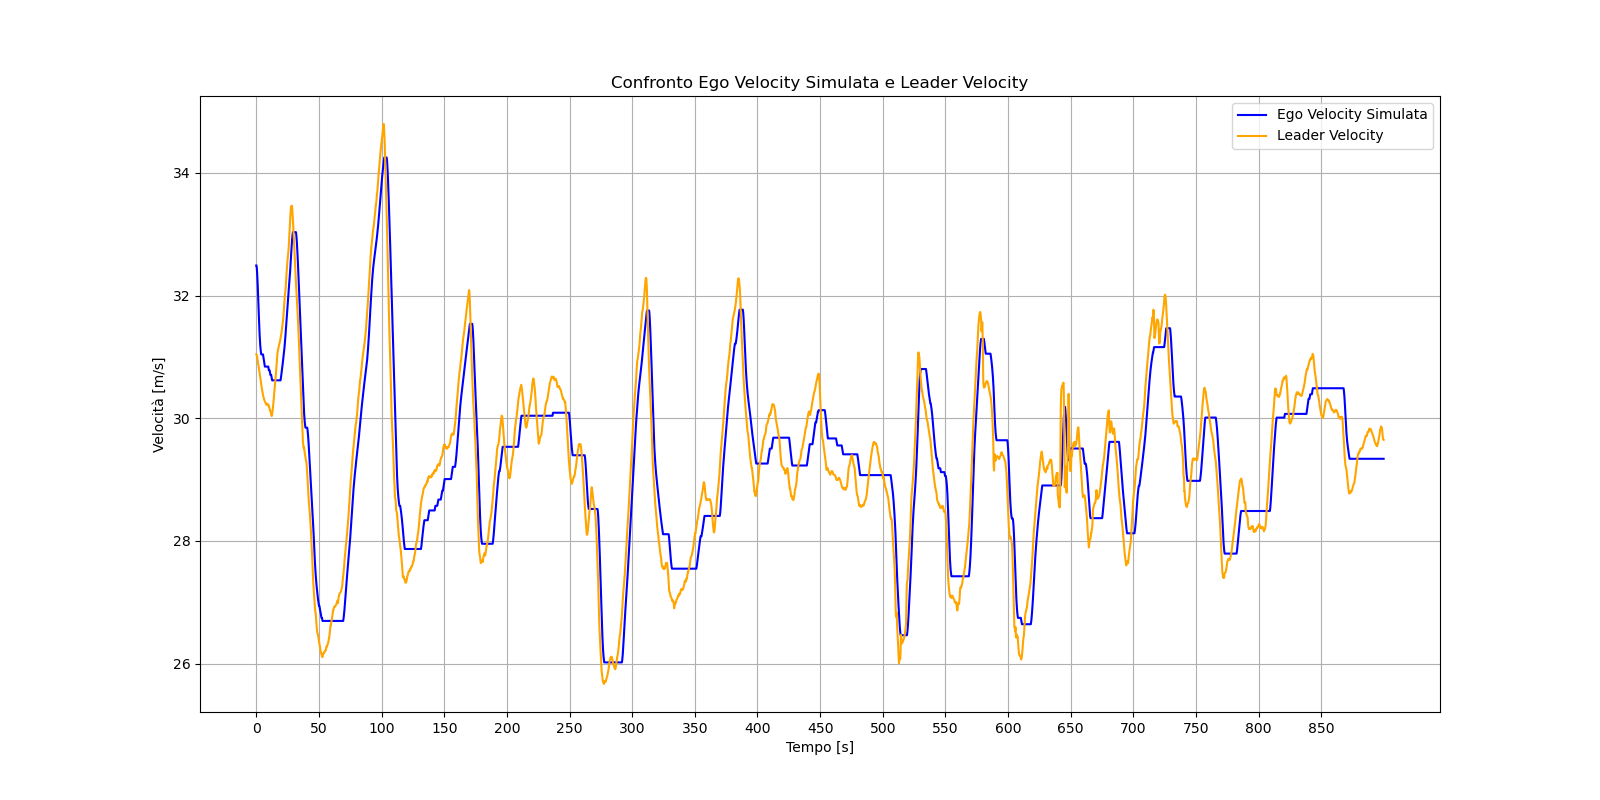
\includegraphics[width=1.25\linewidth]{simulation/bad_weather_ego_comparison/velocity.png}
    }
    \caption{Confronto Ego Velocity Simulata}
    \label{fig:ego_velocity_bw}
\end{figure}
\noindent Anche in questo caso le curve risultano fortemente correlate (coefficiente di Pearson pari a \textbf{0.987}). 
L'unica differenza significativa si osserva nella fase iniziale, dove, in presenza di condizioni atmosferiche 
avverse, il sistema ACC mantiene una velocità inferiore, al fine di aumentare lo spazio dal veicolo che precede.
\clearpage
\noindent Infine, la Figura \ref{fig:space_gap_bw} evidenzia il confronto tra gli \texttt{space\_gap}.
\begin{figure}[H]
    \centering
    \adjustbox{center}{
        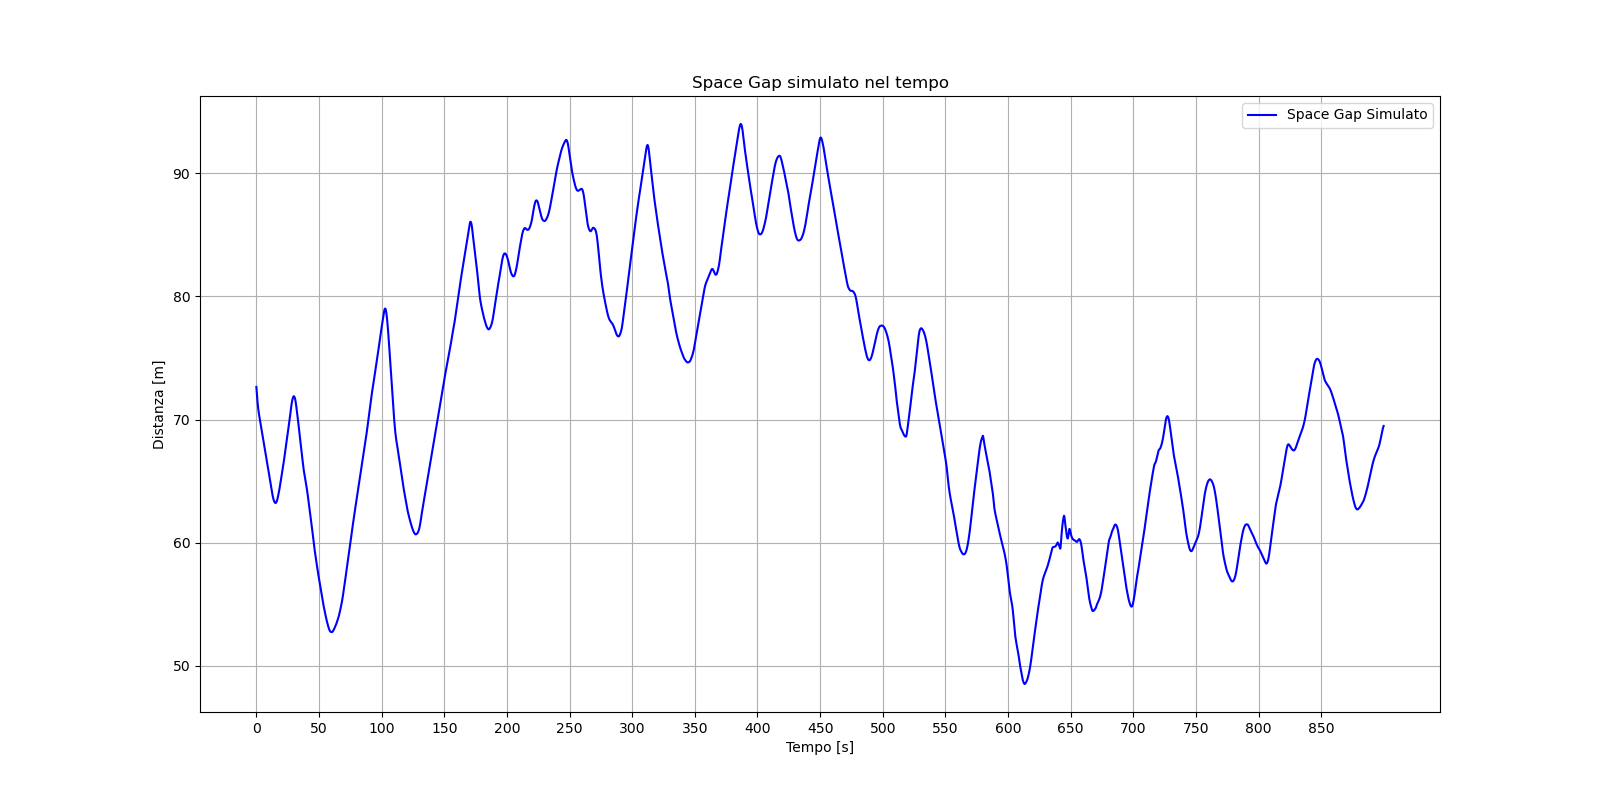
\includegraphics[width=1.25\linewidth]{simulation/bad_weather_ego_comparison/space_gap.png}
    }
    \caption{Confronto Space Gap Simulato}
    \label{fig:space_gap_bw}
\end{figure}
\noindent Come ipotizzato dai grafici precedenti,
in condizioni di bad weather l'ACC aumenta inizialmente la distanza di sicurezza, per poi allinearsi progressivamente 
al comportamento osservato nello scenario di \texttt{good\_weather}. Le due curve risultano dunque simili nella fase centrale e 
finale della simulazione, con una differenza media pari a \(\mu = 56.624 \, \mathrm{m}\) e una deviazione 
standard \(\sigma = 18.734 \, \mathrm{m}\). Questo conferma che l'effetto principale del maltempo si manifesta 
nella fase iniziale della risposta del sistema, mentre sul lungo periodo l'andamento delle due simulazioni tende a convergere.